\documentclass[11pt]{article}
\usepackage{amsmath,textcomp,amssymb,geometry,graphicx,rotating,multirow, listings}

\lstset{breaklines=true}

\def\Name{Sahar Mesri, Sagar Karandikar}
\def\Login{cs150-bw, cs150-bn}

\title{CS150 Checkpoint 3 Proposal, Team 07}
\author{\Name, \texttt{\Login}}
\pagestyle{myheadings}

\begin{document}
\maketitle
\section*{1. Block Diagrams}

\subsection*{Overall System}

\noindent\includegraphics[scale=0.15]{modules/overall.png}

\subsection*{a. Gaussian Filter Banks}

Octave Module:

\noindent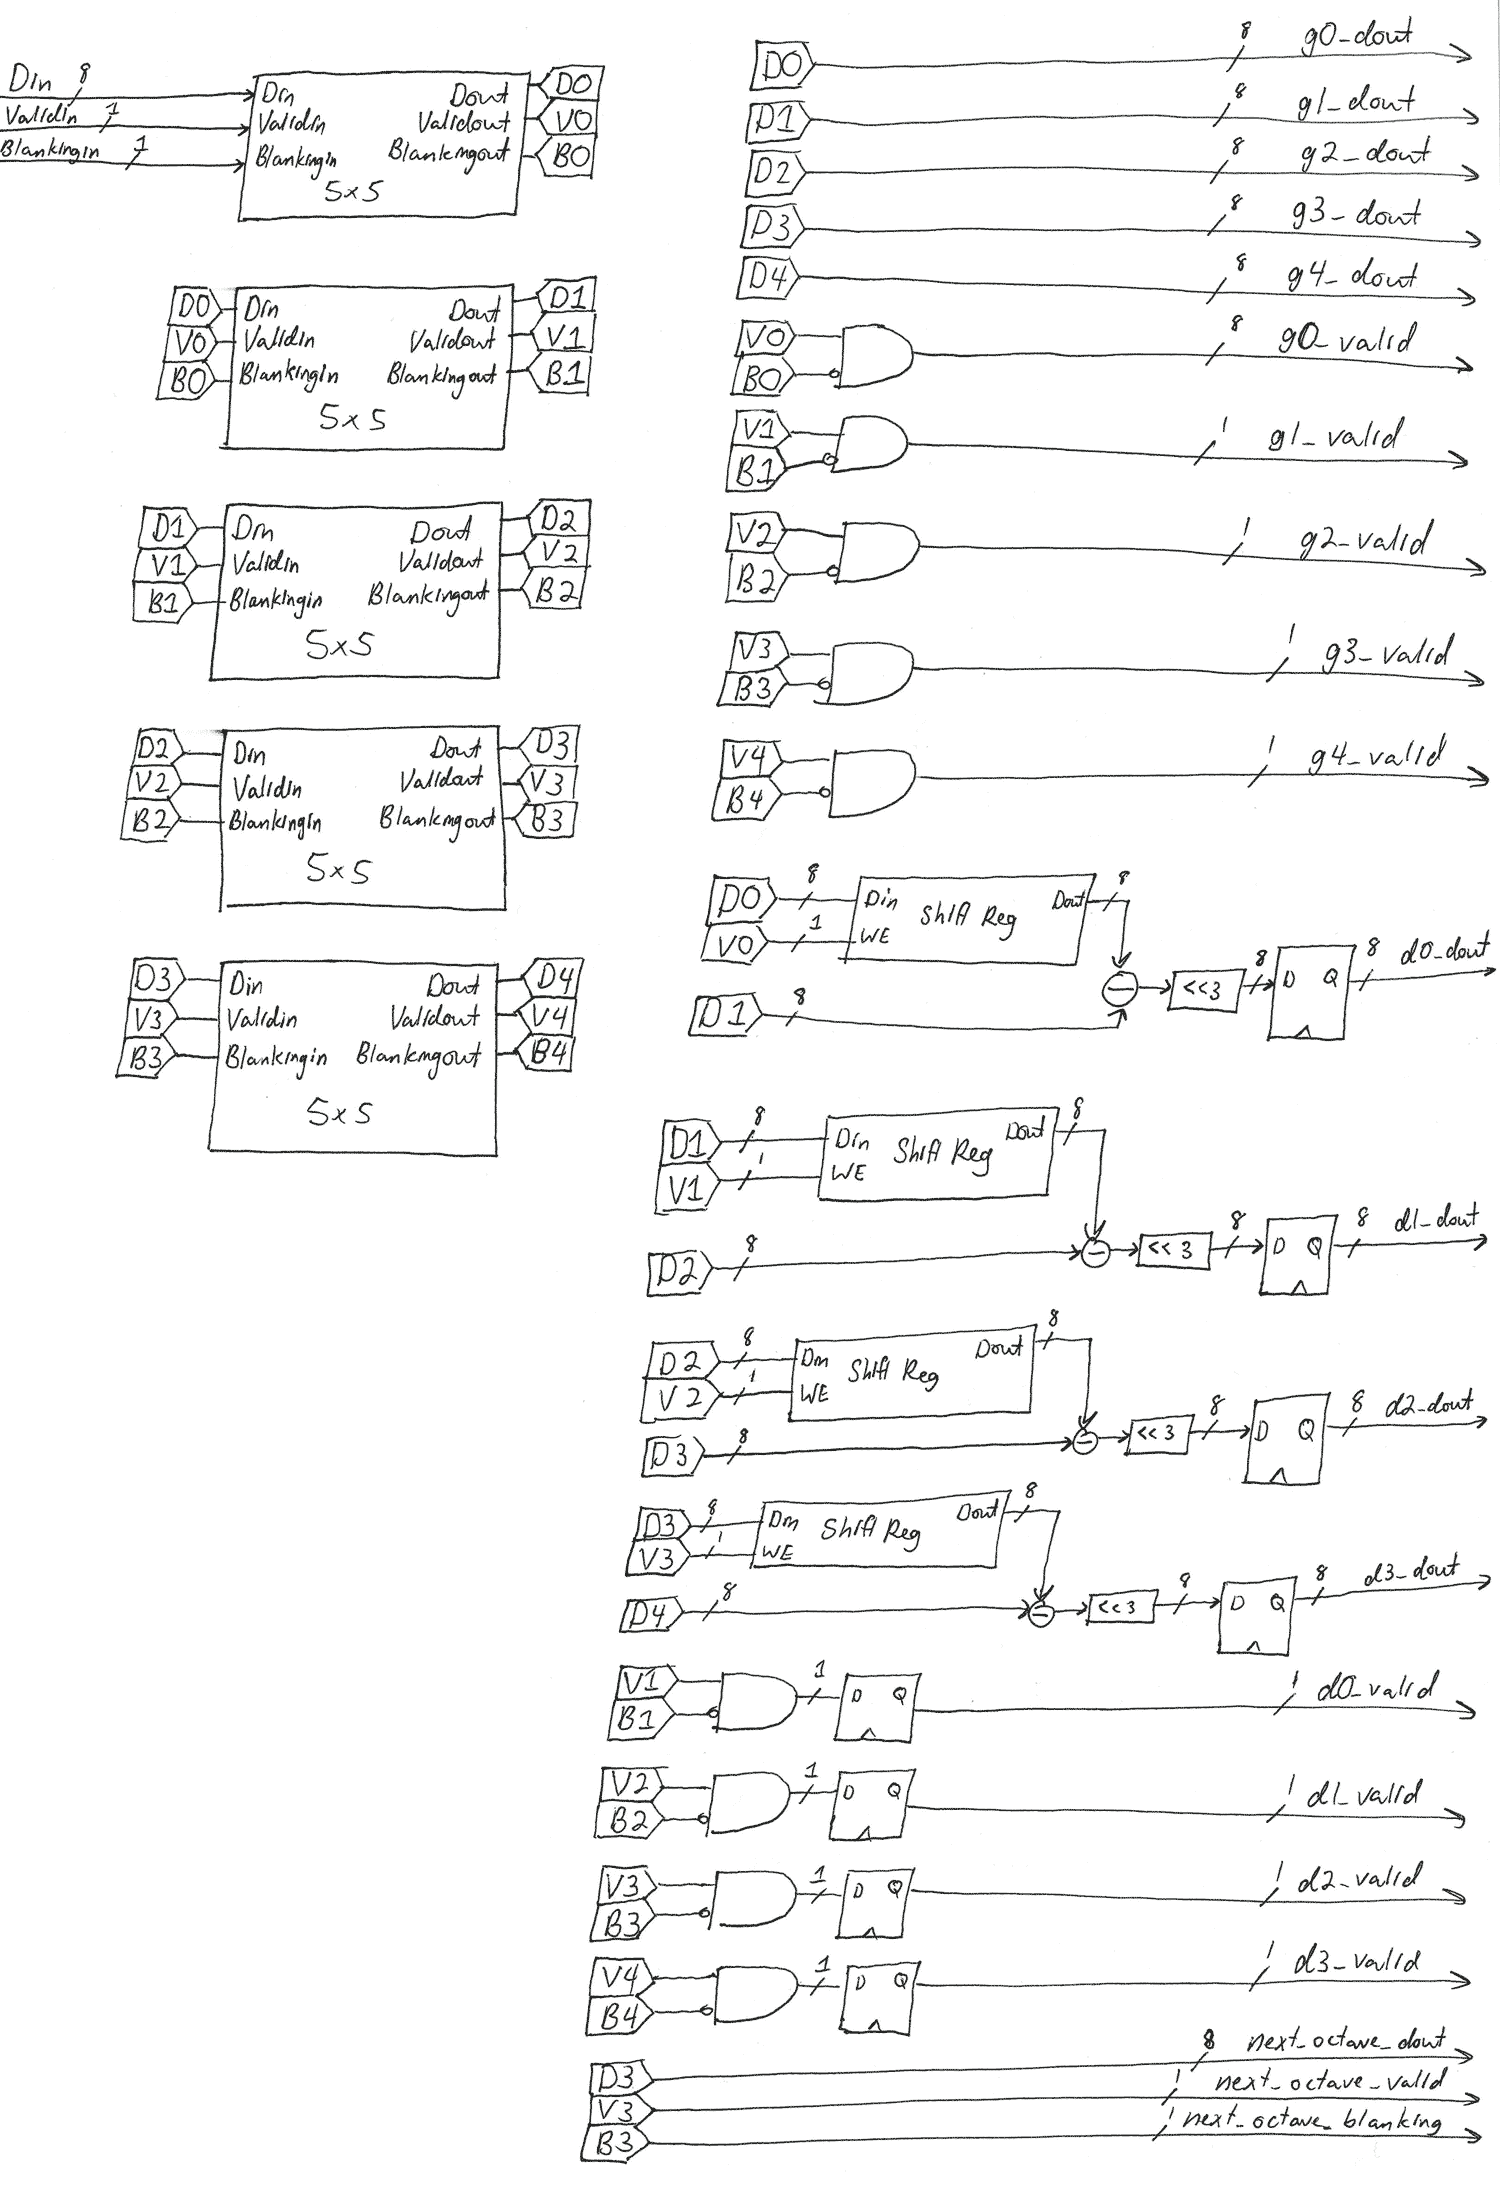
\includegraphics[scale=0.15]{modules/octave.png}

5x5 Window Module:

\noindent\includegraphics[scale=0.15]{modules/5x5window.png}

X Window Module:

\noindent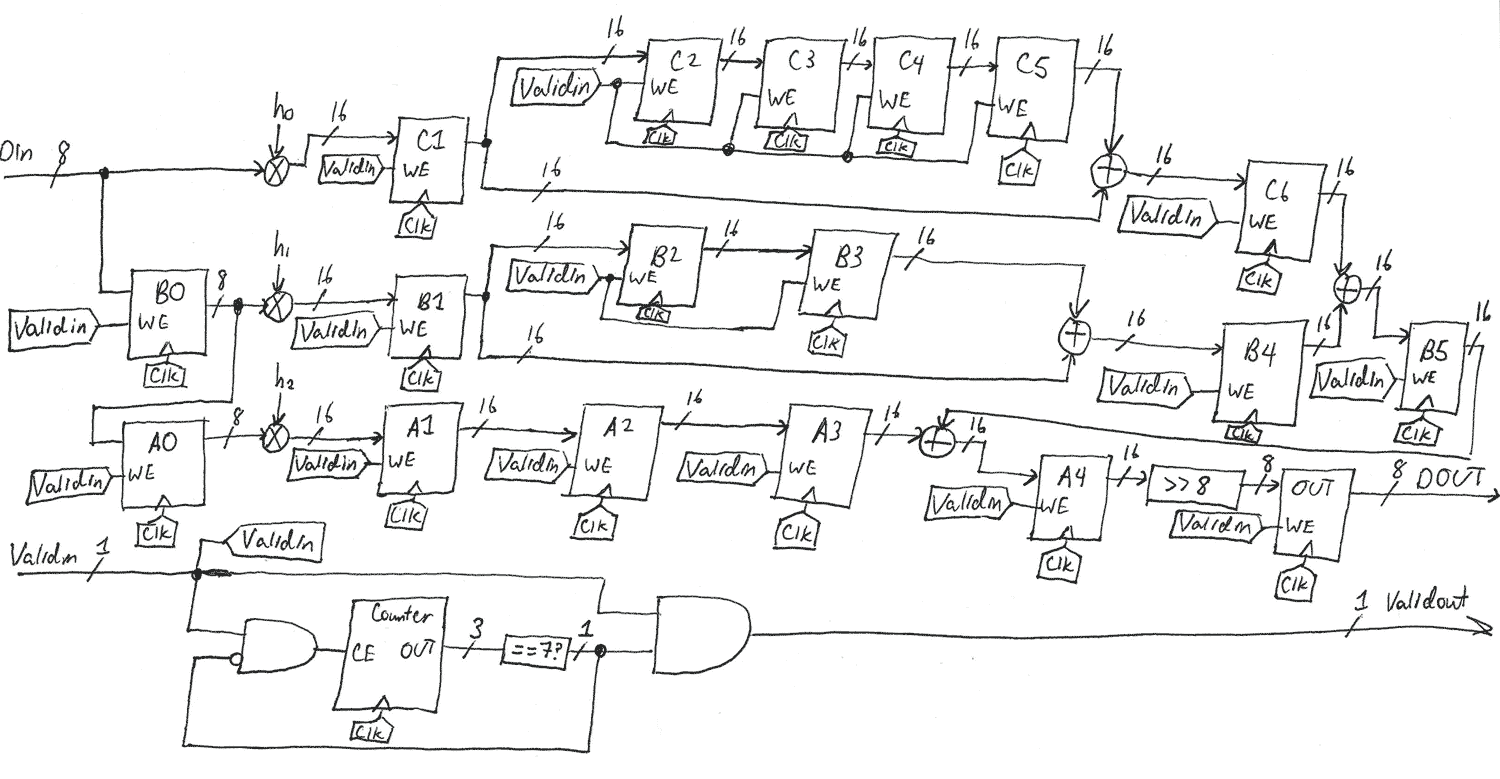
\includegraphics[scale=0.15]{modules/x_window.png}

Y Window Module:

\noindent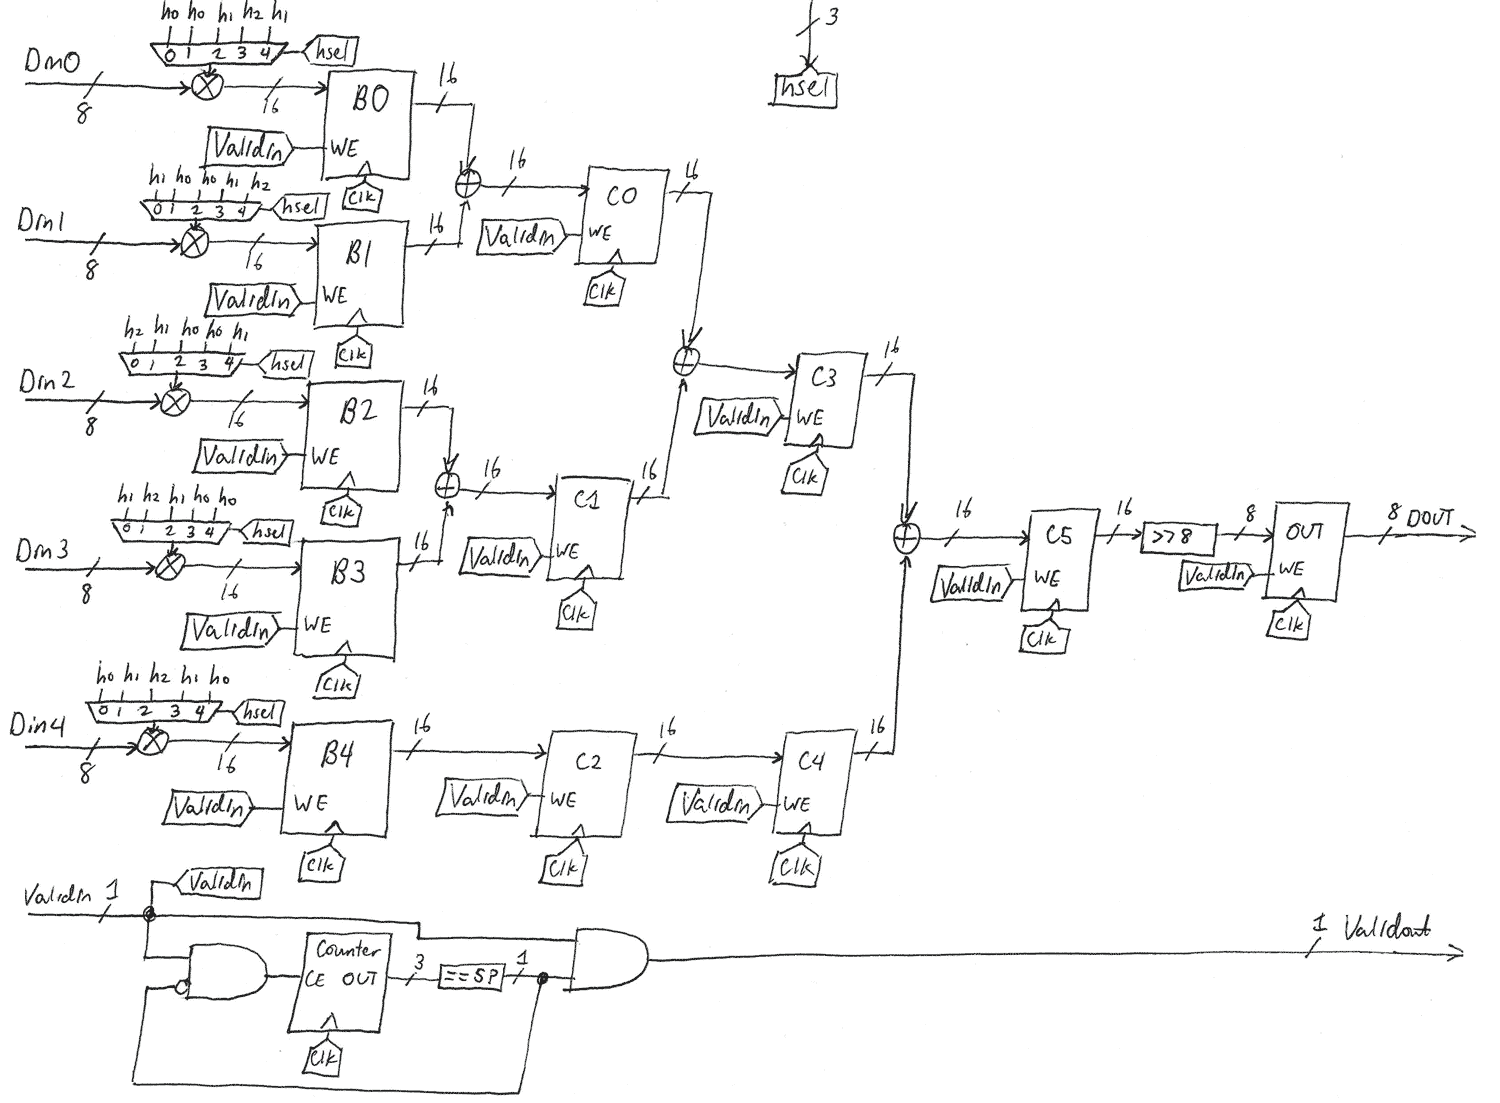
\includegraphics[scale=0.15]{modules/y_window.png}

5 Row Array Module:

\noindent\includegraphics[scale=0.15]{modules/5row.png}

\subsection*{b. Downsampling}

800x600 to 420x320 downsampler (2x + adds padding):

\noindent\includegraphics[scale=0.15]{modules/downsampler2x.png}

420x320 to 210x160 downsampler (2x)

\noindent\includegraphics[scale=0.15]{modules/downsampler2x_simple.png}

\subsection*{c. Upsampling}

\subsection*{d. Interface Connections}

(See overall diagram)

\section*{2. List of Signals}

\subsection*{Datapath Inputs}

\indent8 bit Data In (from VGA controller)

1 bit Valid  (from VGA controller)

1 bit DTACK (from VGA controller)

3 external clocks (not necessarily different clocks, but can be to reduce stalls)

1 bit out\_sel: selects which octave to output if orig/dog = dog

1 bit orig/dog: 0 indicates output VGA input, 1 indicates output dog octave indicated by out\_sel

\subsection*{Datapath Outputs}

8 bit Data Out

1 bit Valid Out

18 bit Address Out (from Address Generator block)

1 bit output clock (for checkpoint 2 write clock)

\section*{3. RT Language Description}

\subsection*{X Window Module}
\begin{lstlisting}

while(true){
    if(ValidIn) {
        B0 <- Din, A0 <- B0, C1 <- h0*Din, B1 <- h1*B0, A1 <- h2*A0, C2 <- C1, C3 <- C2, C4 <- C3, C5 <- C4, C6 <- C5 + C1, B2 <- B1, B3 <- B2, B4 <- B3 + B1, B5 <- C6 + B4, A2 <- A1, A3 <- A2, A4 <- B5 + A3, Out <- 1/5 * A4, Counter <- Counter + 1 if Counter != 7;
    }
}
\end{lstlisting}


\section*{4. Controller State Diagram}

\section*{5. Testbench Outline}

\end{document}
